\setlength{\baselineskip}{20pt}
\chapter{基于迁移和特征工程的联邦学习CAN异常检测}
\label{cha:chap3}

\section{相关工作和技术介绍}

\subsection{联邦迁移学习}
联邦学习是保护输入隐私的分布式计算范式,可以实现各个客户端数据不共享的条件下的协同计算。具体来说,服务器与各个客户端通过中间结果的多轮交互来获得计算结果,在整个计算过程中,客户端的数据始终存储在本地,同时其他客户端和服务器对该客户端的数据没有任何访问权限。在客户端知情并且同意隐私政策的前提下,联邦学习满足数据最小化原则。在每轮迭代过程中,客户端仅为特定的计算任务传输必要的更新,同时,服务器仅短暂存储中间结果以即时完成聚合,并仅发布最终的计算结果。然而,现有工作表明,攻击者可以依据中间结果获得原始数据的一些信息,因此,联邦学习还需结合安全多方计算或同态加密等来增强计算过程的保密性,并结合差分隐私来增强结果发布的匿名性。目前,谷歌、微众银行、达摩院及百度等机构发布了联邦学习开源框架,并且联邦学习已经在政务、金融和医疗等场景中得到应用。

\begin{figure}[htb]
\centering
    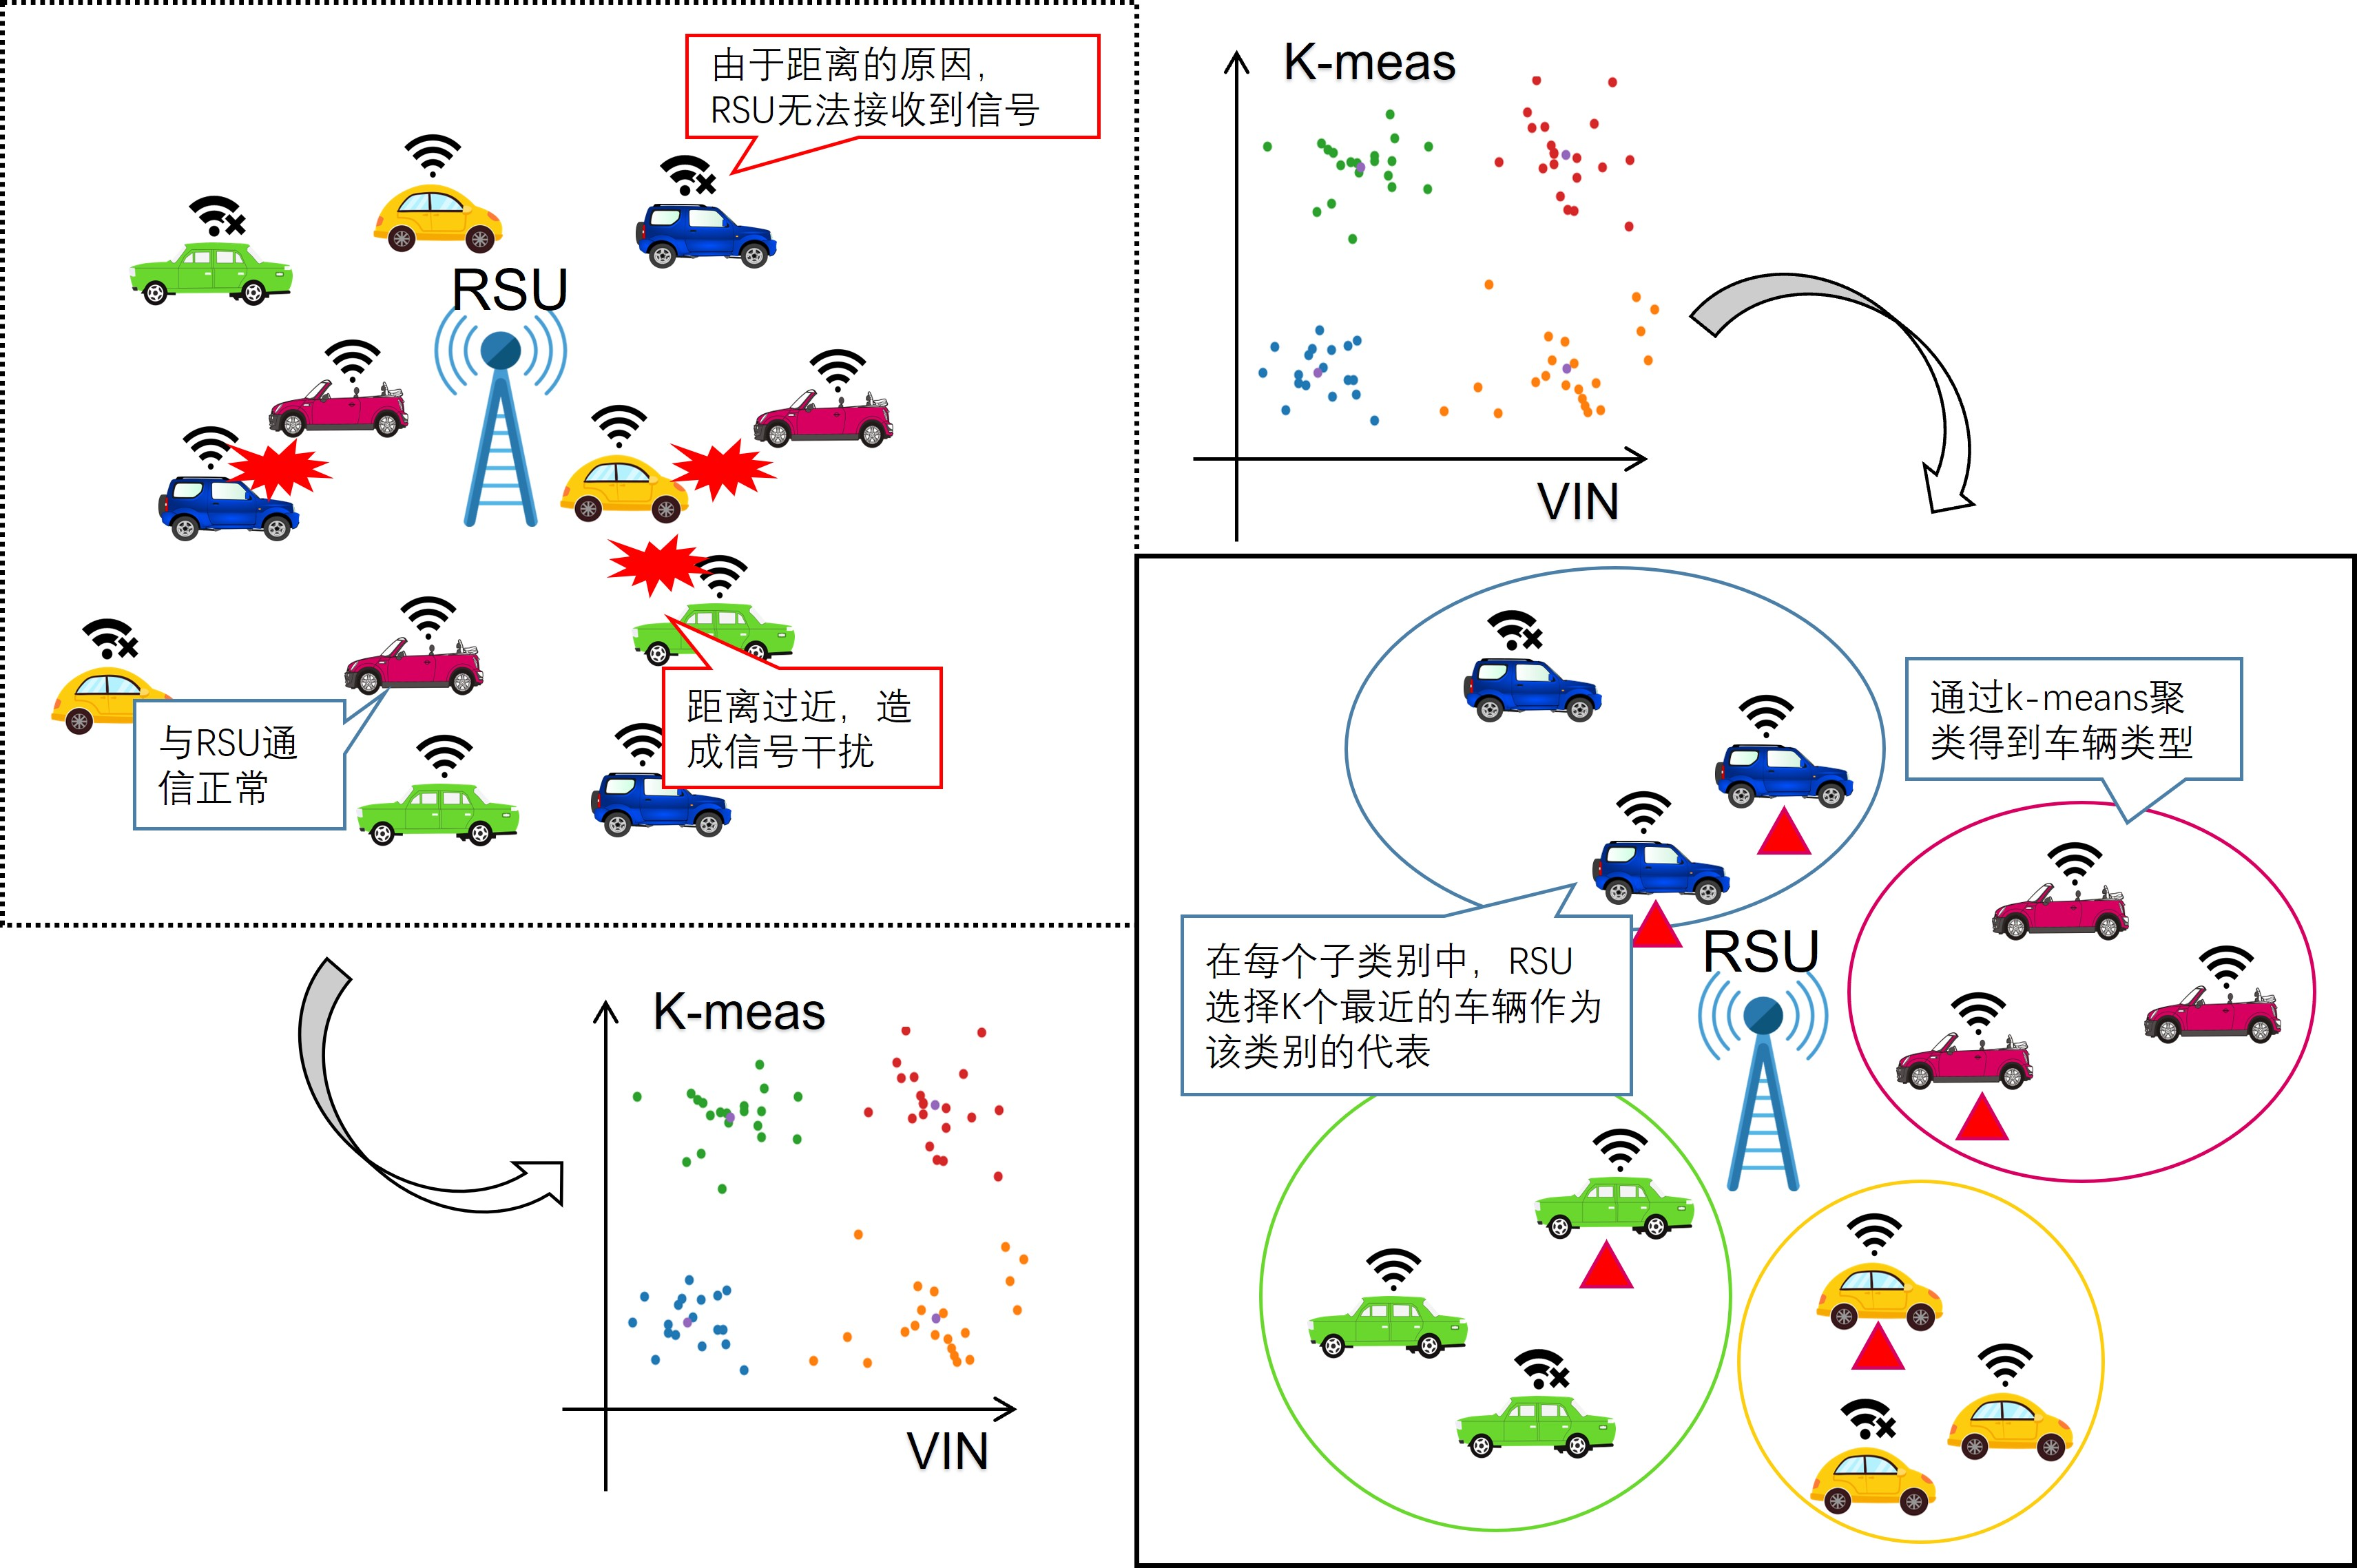
\includegraphics[scale=0.5]{figures/figure1.jpg}
    % \caption{FL-vgg16 Confusion Matrix}
    \caption{隐私保护计算的主要技术与三大隐私保证的对应关系}
    \label{fig:Cluster the cars in the region}
\end{figure}

\subsection{特征工程}

\subsection{汽车总线}

\section{基于迁移和特征工程的联邦学习CAN异常检测}\label{sec:HC}

本节提出了一种基于迁移和特征工程的联邦学习CAN异常检测的设计框架,该框架由三层组成,分别是:RSU(Road Side Unit,路侧单元)与MEC(Multi-access Edge Computing,多接入边缘计算)层,车与RSU层,车与车层。在该框架中,车联网中的车辆都装备了ECU(Electronic Control Unit,电子控制器单元)、OBUs和各种应用单元,实现了车辆之间和车辆与RSU之间的通信。MEC作为边缘计算的平台,提供了强大的计算能力,负责对来自不同RSU的联邦模型进行聚合更新和数据存储。RSU作为车联网的核心节点,负责本地模型的训练、数据的收集和清洗、异常检测的执行等功能,并将检测结果反馈给所属区域的车辆。当车辆进入RSU的服务范围时,可以主动向RSU发送检测请求,RSU则会收集车辆传输的CAN数据,并对其进行清洗和模型训练。

\subsection{车辆与RSU之间的数据传输}

\begin{figure}[htb]
\centering
    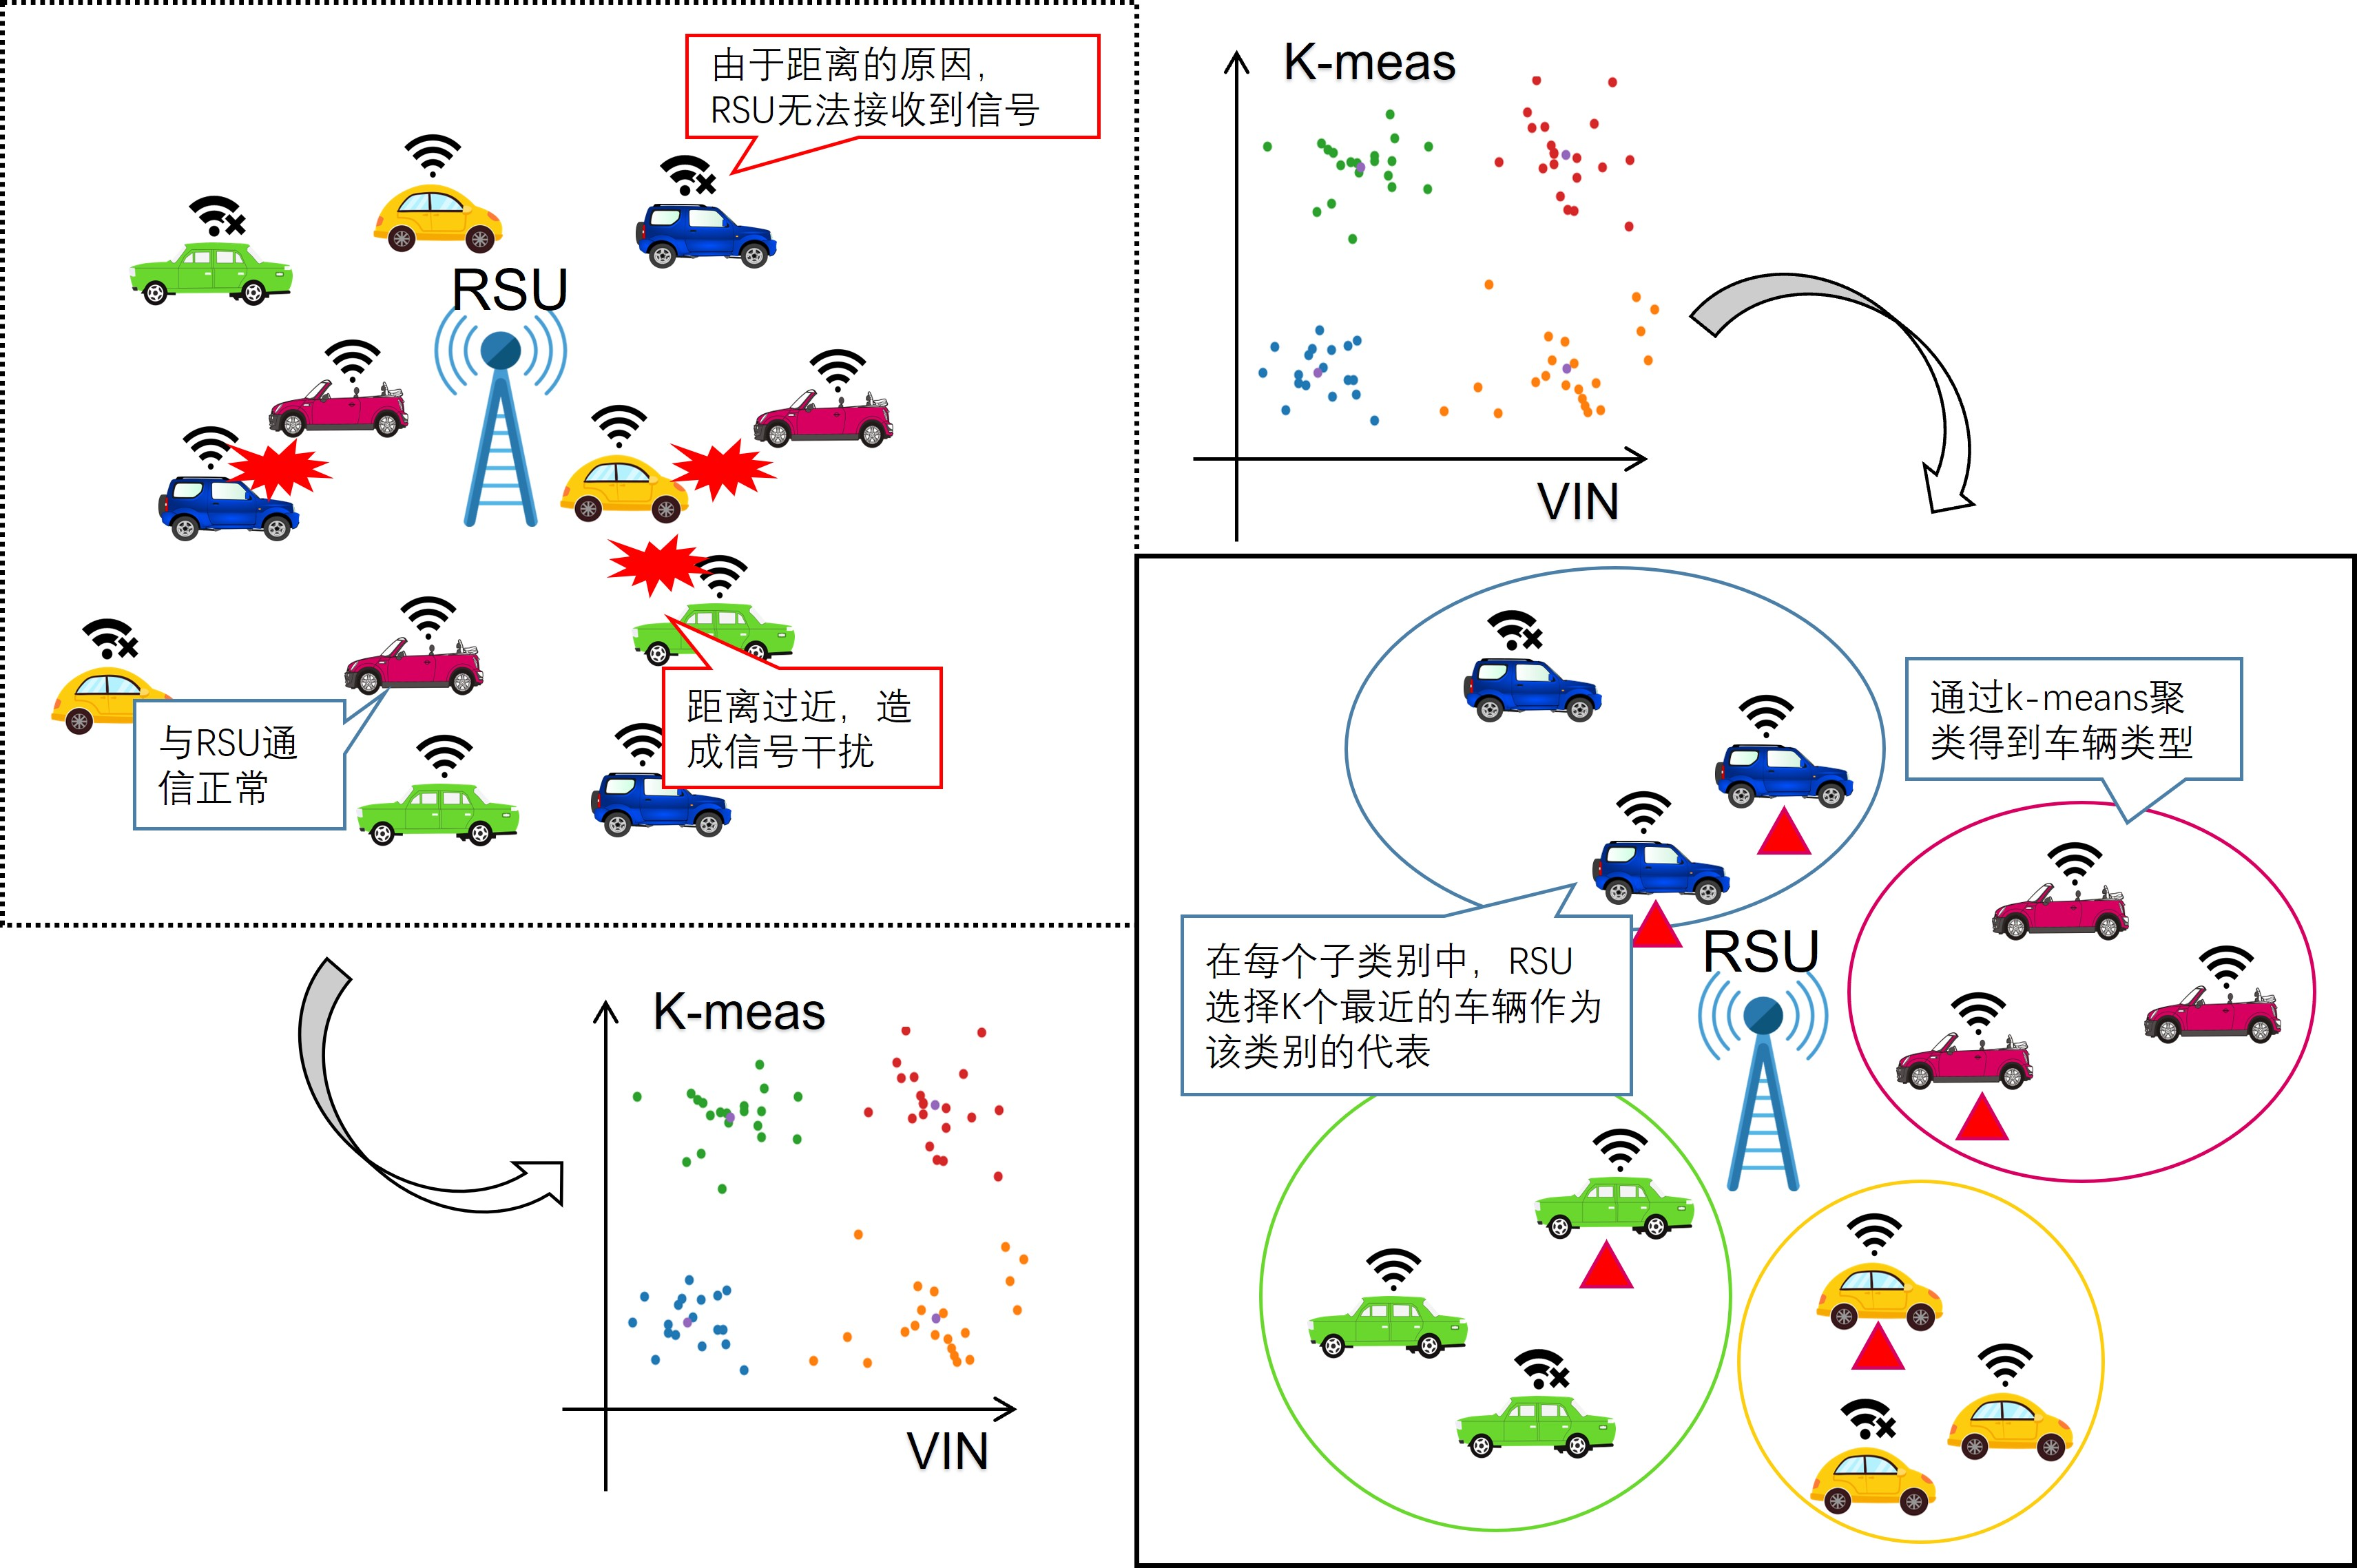
\includegraphics[scale=0.5]{figures/figure1.jpg}
    % \caption{FL-vgg16 Confusion Matrix}
    \caption{对区域内的车进行聚类}
    \label{fig:Cluster the cars in the region}
\end{figure}

本节考虑了车辆的动态性对联邦学习的影响,分析了车辆移动对RSU数据收集质量的影响(如传输延迟、消息碰撞或中断等)。由于入侵检测的目的是保护车辆的安全而不是RSU的安全,因此本节假设系统中的车辆都是积极的参与者,只有在自身条件允许时,才会将车辆识别码(Vehicle Identification Number,VIN)和位置信息传输给RSU。如图\ref{fig:Cluster the cars in the region}所示,RSU根据车辆识别码(Vehicle Identification Number,VIN)对区域内的车辆进行K-means聚类,假设可以将车辆分为$N$个类别,RSU根据欧几里得公式\ref{math:k-means},从每个类别中选择$k \geq 1$辆车作为本地数据来源,共计$kN$辆车。图中所示的情况是$N=4$,$k=2$。实际上,RSU将从每个类别中选择$max(1,k)$辆车,以保证每个类别至少有一辆车参与数据传输。

\begin{equation}
\begin{array}{l}
|AB|=\sqrt{(x_2-x_1)^2+(y_2-y)^2+(z_2-z_1)^2}\\
k\to\max(1,k)
\end{array}
\label{math:k-means}
\end{equation}

% 该模型将运行在智能车上,智能车的主要任务是自动巡航,因此不希望入侵检测占用大量的计算资源。轻量级的DL模型和欠采样技术通常应用于样本不均衡且数据集足够时,通过减少多数类的样本数以此获得类别均衡的数据集。当RSU接收到车辆的数据量超过自身内存的50\%时,会启动数据欠采样操作。欠采样方法集合中的Near Miss\cite{Zhang03}会根据多数类实例与少数类实例之间的距离来选择样本。该技术有三种版本,分别称为NearMiss-1,NearMiss-2和NearMiss-3。选用NearMiss-1时,会从多数类中选择那些与少数类中三个最接近示例的平均距离最小的示例。紧接着对数据进行非线性转换,这里本节选择的是yeo-Johnson\cite{yeo},其转化如公式\ref{math:yeo}所示。

% \begin{equation}
% \begin{aligned}
% x_i^{(\lambda )}=\begin{cases}
%  [(x_i+1)^\lambda -1] / \lambda  & \text{ if } \space  \lambda \ne 0,x_i \ge 0 \\
%  ln(x_i)+1  & \text{ if } \space  \lambda =  0,x_i \ge 0 \\
%  -[(-x_i+1)^{2-\lambda } -1] / (2-\lambda ) & \text{ if } \space  \lambda \ne 2,x_i <  0\\
%  -ln(-x_i+1) & \text{ if } \space  \lambda =  2,x_i < 0
% \end{cases}
% \label{math:yeo}
% \end{aligned}
% \end{equation}

% 文献\cite{A_Transfer_Learning_and_Optimized_CNN_Based_Intrusion_Detection_System_for_Internet_of_Vehicles}中选择的是quantile Transformer将数据转化为$0-1$中的均匀分布。然而,在机器学习领域中,具有正态分布形式的特征变量是大多数算法所期望的输入形式,幂转化可以将任何形式的分布转化为高斯分布,能够使方差稳定,减少偏度保持对称性。但是yeo-Johnson不能保证输出的值是一个0到1之间的值,所以在这之后本节又加上了如公式\ref{math:14}所示的min-max标准化。

为了在智能车上实现入侵检测,本节引入特征工程思想,首先,采用轻量级的DL模型和欠采样技术,以降低计算资源的消耗和解决样本不均衡的问题。欠采样技术的原理是通过减少多数类的样本数量,使数据集的类别分布更加平衡。本节引入特征学习思想,首先使用一种基于距离的欠采样方法,即Near Miss\cite{Zhang03},该方法有三种版本,分别是NearMiss-1,NearMiss-2和NearMiss-3。本节选择了NearMiss-1,其算法是从多数类中选择那些与少数类中最近的三个样本的平均距离最小的样本。当RSU接收到的车辆数据量超过其内存的50\%时,就会对数据进行欠采样处理。其次,为了使数据更适合DL模型的输入,本节还对数据进行了非线性变换,即yeo-Johnson\cite{yeo}变换,其公式如下:

\begin{equation}
\begin{aligned}
x_i^{(\lambda )}=\begin{cases}
 [(x_i+1)^\lambda -1] / \lambda  & \text{ if } \space  \lambda \ne 0,x_i \ge 0 \\
 ln(x_i)+1  & \text{ if } \space  \lambda =  0,x_i \ge 0 \\
 -[(-x_i+1)^{2-\lambda } -1] / (2-\lambda ) & \text{ if } \space  \lambda \ne 2,x_i <  0\\
 -ln(-x_i+1) & \text{ if } \space  \lambda =  2,x_i < 0
\end{cases}
\label{math:yeo}
\end{aligned}
\end{equation}

yeo-Johnson变换是一种幂变换,可以将任何分布的数据转换为正态分布,从而使数据的方差稳定,减少偏度,保持对称性。这些特性有利于提高机器学习算法的性能。然而,yeo-Johnson变换不能保证输出的数据在$0-1$之间,因此本节在变换后还对数据进行了min-max标准化,其公式如下:

\begin{equation}
\begin{aligned}
x_i'=\frac{x_i-\min(x)}{\max(x)-\min(x)}
\label{math:14}
\end{aligned}
\end{equation}

最后,使用min-max标准化将数据缩放到$0-1$之间,使数据的范围更加一致,避免因为数据的量纲不同而影响模型的训练效果。文献\cite{A_Transfer_Learning_and_Optimized_CNN_Based_Intrusion_Detection_System_for_Internet_of_Vehicles}中使用了quantile Transformer将数据转换为$0-1$之间的均匀分布,但本节认为正态分布更符合数据的实际情况,此时,所有的CAN数据都将落到0-255之前,由于数据的特殊性,可以将其由十六进制的字节码转化为图片数据,详细见本文的实验设置部分。

\subsection{RSU的DL模型选择}

\begin{figure}[htb]
\centering
    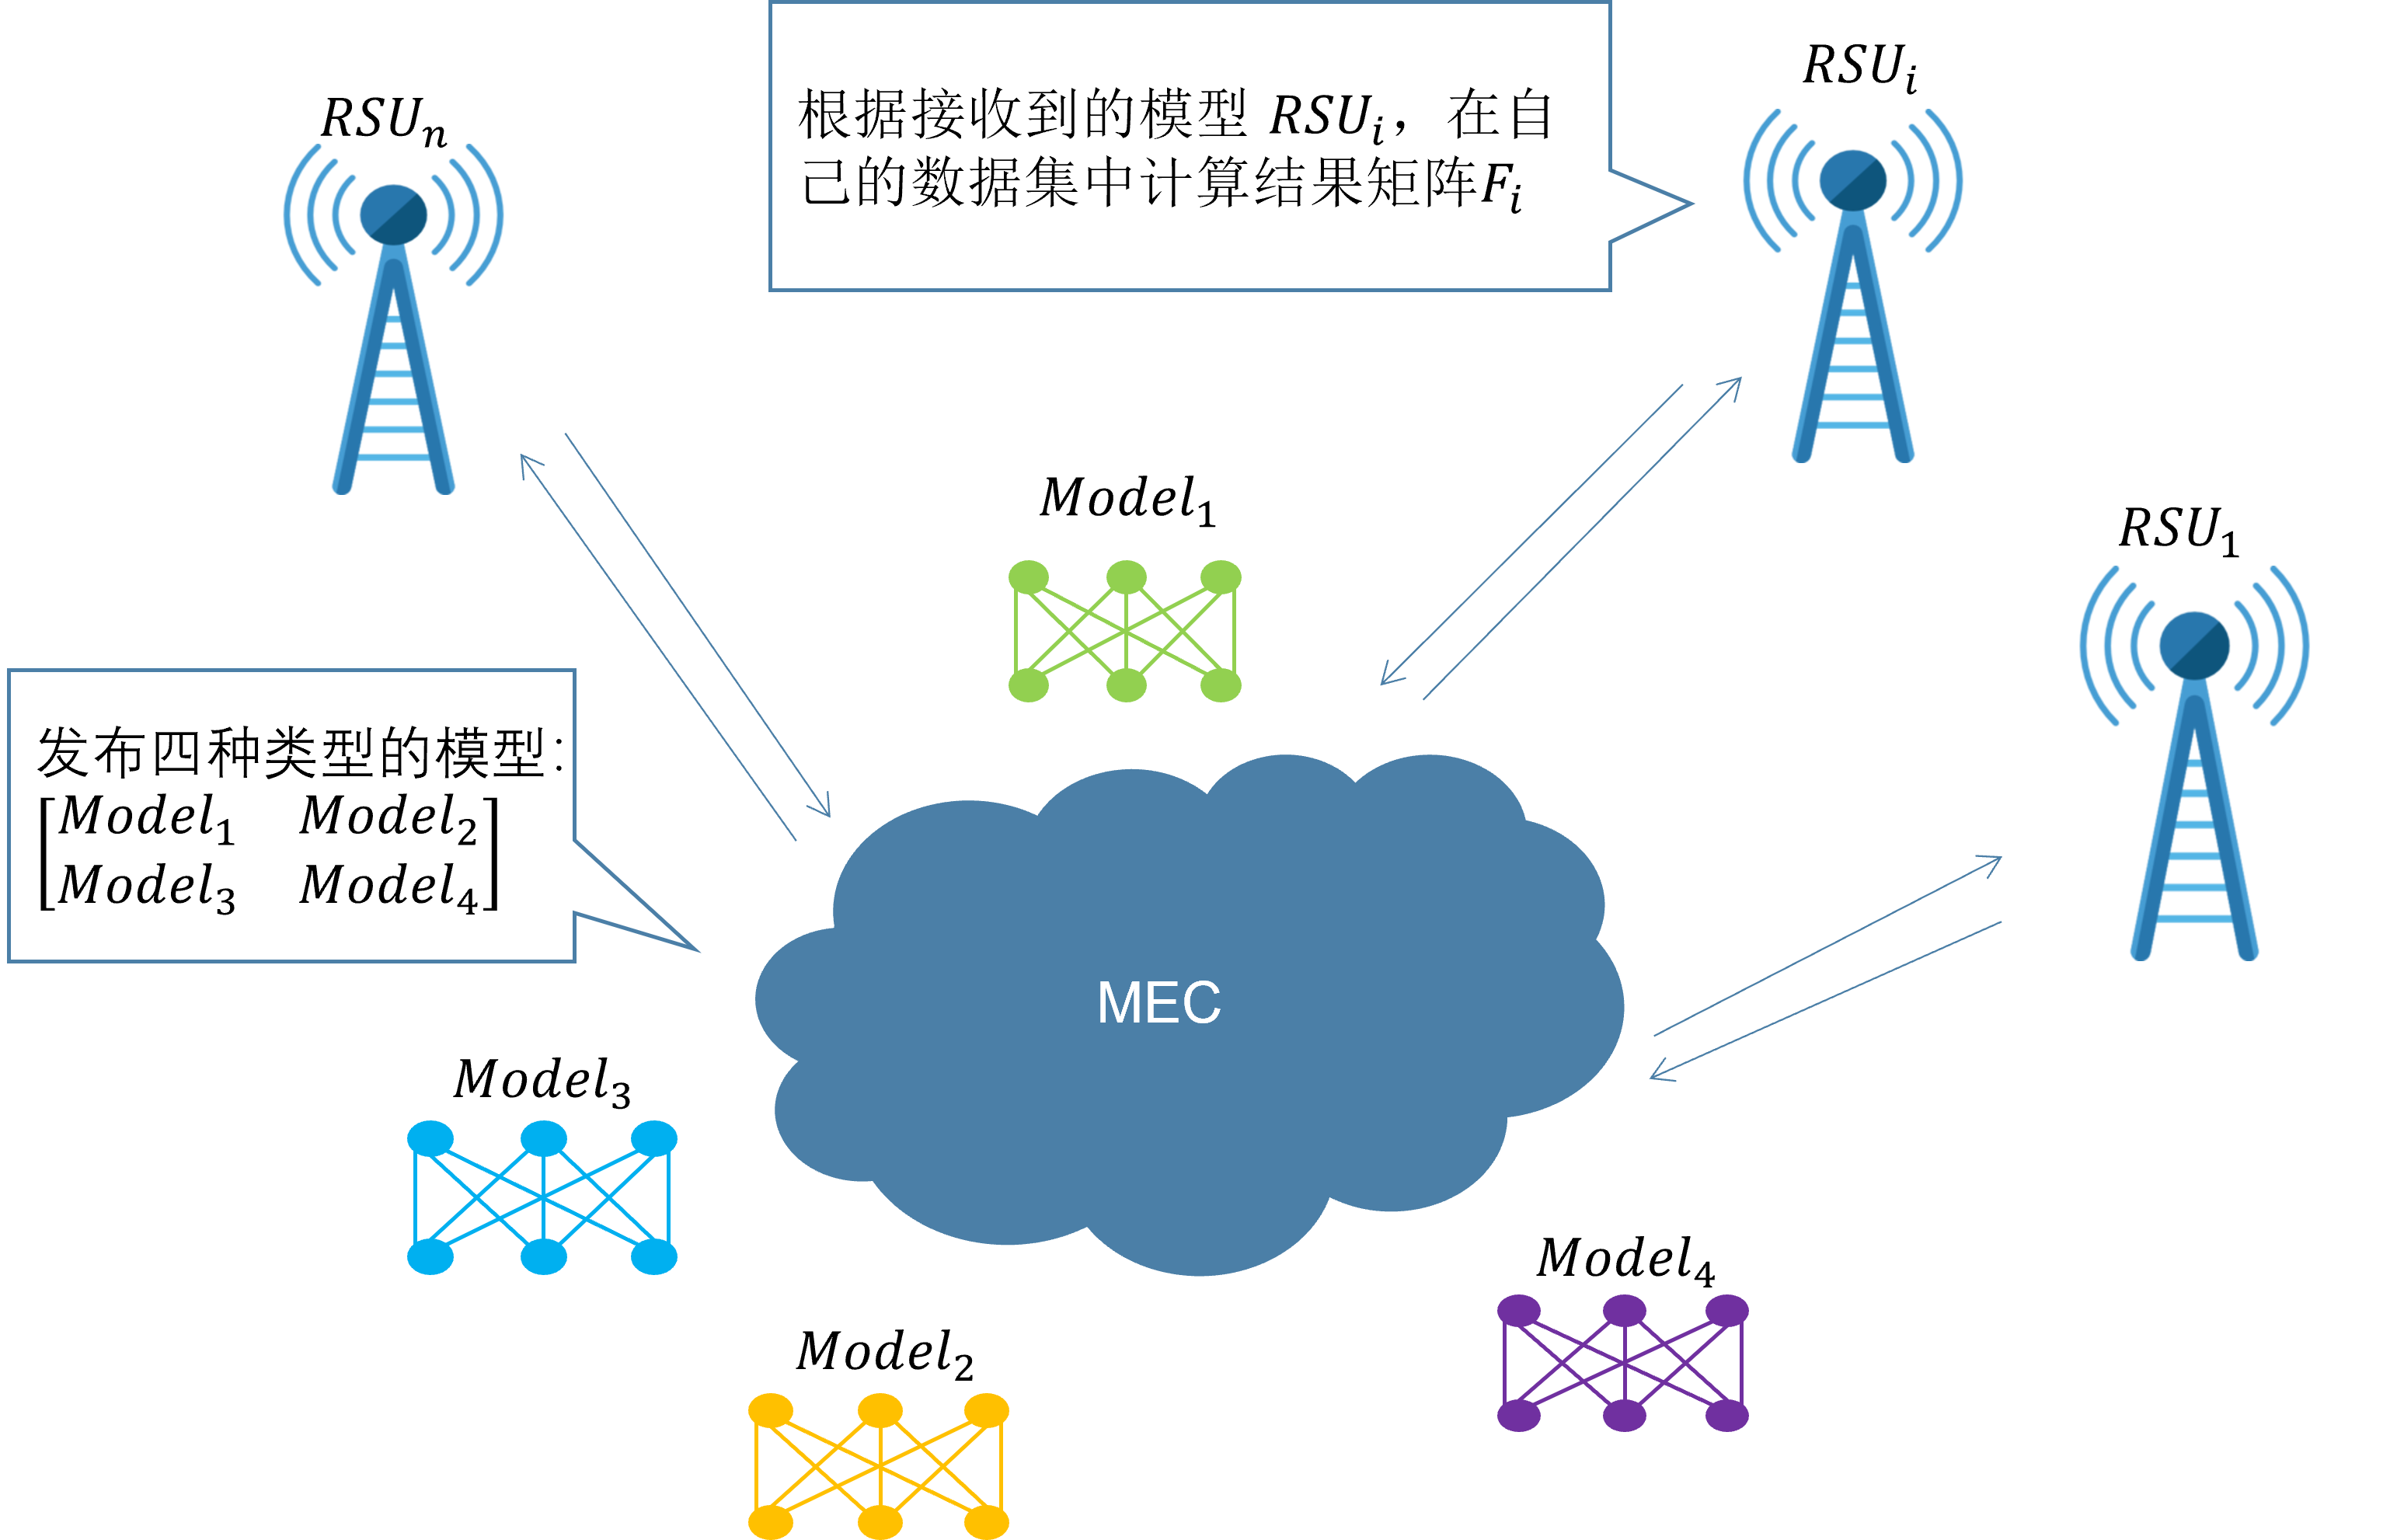
\includegraphics[scale=0.6]{figures/figure2.png}
    % \caption{FL-vgg16 Confusion Matrix}
    \caption{对区域内的车进行聚类}
    \label{fig:Cluster the cars in the region}
\end{figure}

本节研究了在移动边缘计算(MEC)环境下,如何为不同类型的路侧单元(RSU)提供个性化的深度学习(DL)模型,以实现车辆入侵检测的联邦学习任务。MEC作为系统的中心节点,负责模型的聚合与分发。由于RSU的种类繁多,不同厂商生产的RSU所配备的软硬件资源不同,同时,不同地点的RSU接收的CAN数据量也不同,例如位于城市主干道上的RSU接收的数据将远远多于乡镇等支线上的数据。因此,本节需要为不同地方的RSU提供更加适合其数据特征和资源条件的模型。

为了解决这一问题,本节引入了迁移学习的思想,利用多个领域的共享知识来建立有效的模型。迁移学习的优势在于,它可以利用已有的大量数据训练出一个好的模型,然后将其作为联邦学习任务的初始模型,从而减少训练时间和资源消耗。本节在MEC中集成了四类预训练后的DL模型,分别是CNN、VGG16、ResNet18、AlexNet。在系统启动的初期,MEC会将这四类模型下发给选中的$\alpha$个RSUs。

设第$i$个RSU为$R_i$,则$R_i$将采用四款模型在本地数据集上进行训练,将模型收敛后得到的更新梯度$g_k,k\in[1,4]$和F1得分$f_k,k \in[1,4]$返回给MEC,其中$g_k$与$f_k$一一对应,表示第$k$个模型训练得到的值。F1得分是一种衡量模型分类性能的指标,其计算公式如公式\ref{math:15}所示。$F'_i$表示为$R_i$的临时结果矩阵,则$F'_i$如公式\ref{math:7}所示。
\begin{equation}
    \begin{aligned}
    F'_i=\begin{bmatrix} f_1 & g_1 \\ f_2 & g_2\\f_3 &  g_3 \\f_4 &  g_4 \end{bmatrix}
    \end{aligned}
    \label{math:7}
\end{equation}
为了选择最适合$R_i$的模型,本节定义了一个系数矩阵$\theta $,设定四个资源相关参数:最大训练时间$t$,最小loss值$l$,模型大小$u$,训练所需CPU性能$c$。对于CNN、VGG16、ResNet18、AlexNet这四类模型来说,最大训练时间$t$,模型大小$u$,训练所需CPU性能$c$都各不相同,而最小loss值$l$均一样。同时定义一个放缩函数$\mathcal{F}, $使得$\mathcal{F}(t),\mathcal{F}(l),\mathcal{F}(u),\mathcal{F}(c) \in (0,1]$,由于本节希望这四个值都越小越好,则可以得到公式\ref{math:11}:
\begin{equation}
    \begin{aligned}
    \theta =\begin{bmatrix}
     \mathcal{F}(t_1)\mathcal{F}(l)\mathcal{F}(u_1)\mathcal{F}(c_1) \\
     \mathcal{F}(t_2)\mathcal{F}(l)\mathcal{F}(u_2)\mathcal{F}(c_2) \\
     \mathcal{F}(t_3)\mathcal{F}(l)\mathcal{F}(u_3)\mathcal{F}(c_3) \\
     \mathcal{F}(t_4)\mathcal{F}(l)\mathcal{F}(u_4)\mathcal{F}(c_4) 
    \end{bmatrix}=\begin{bmatrix}
     \theta_1 \\ \theta_2 \\ \theta_3 \\  \theta_4
    \end{bmatrix}
    \end{aligned} 
    \label{math:11}
\end{equation}
因此最终的结果矩阵$F_i$如公式\ref{math:12}所示:
\begin{equation}
    \begin{aligned}
    F_i=\begin{bmatrix} f_1/\theta_1  & g_1 \\ f_2/\theta_2  & g_2\\f_3/\theta_3  &  g_3 \\f_4/\theta_4 &  g_4 \end{bmatrix}
    \end{aligned} \label{math:12}
\end{equation}

\subsection{MEC的联邦学习}

\begin{figure}[htb]
\centering
    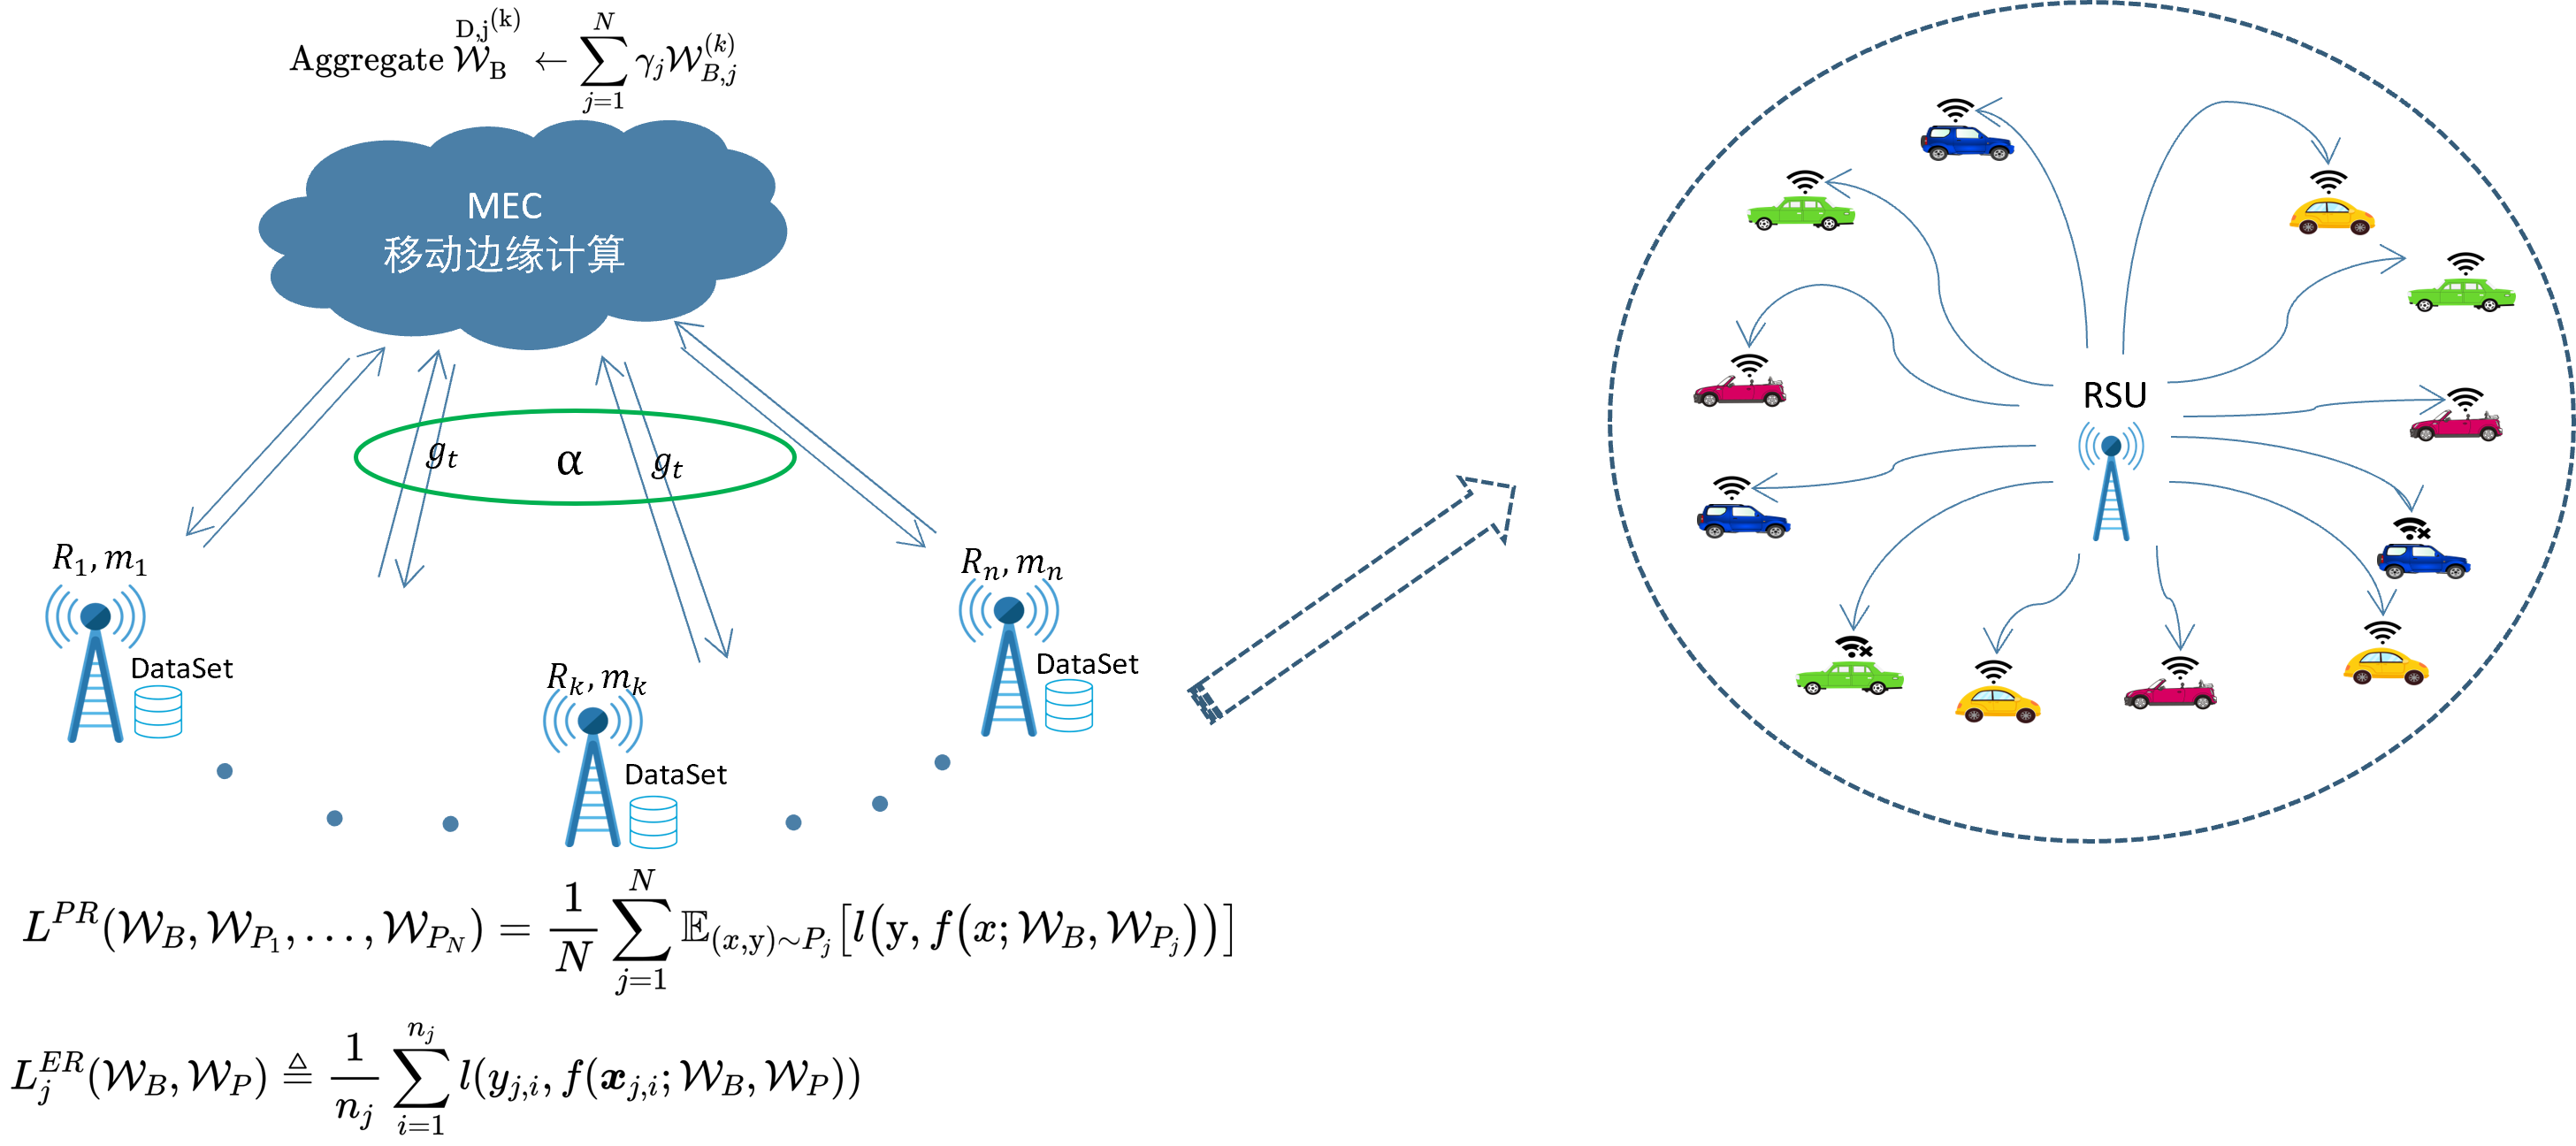
\includegraphics[scale=0.65]{figures/chapter3/chapter3.png}
    % \caption{FL-vgg16 Confusion Matrix}
    \caption{对RSU进行聚类}
    \label{fig:Cluster the cars in the region}
\end{figure}

本节研究了在移动边缘计算(MEC)环境下,如何为不同类型的路侧单元(RSU)提供个性化的深度学习(DL)模型,以实现车辆入侵检测的联邦学习任务。MEC作为系统的中心节点,负责模型的聚合与分发。MEC收到所有RSU传来的结果矩阵后,会得到集合$F=\{F_1,F_2,\dots,F_n\}$。MEC将根据$F$进行二次聚类,将区域内的RSU分配到四类模型中。
% 对于每一个小分类,使用FedPer\cite{Federated_learning_with_personalization_layers}算法,进行全局模型训练。FedPer算法的核心思想是将待训练的模型分为“基础+个性化层”,基础层可以作为共享层捕捉群体的智慧,而个性化层可以作为任务特定层捕捉客户端特定方面。

取$F_{sum}$中最大值$F_{s_k}= MAX(F_{sum})$对应的模型作为联邦学习系统中的最终模型$M_{select}$,同时得到对应梯度$ g_{select}= G_{s_k}$。设第$t$轮,MEC上的全局模型为$M_{i_t}$,参与更新的RSU集合为$R=\{R_1,R_2,\dots,R_n\}$,$R_k \in R$,对应的数据索引集大小为$m_k$,所有参与方的数据集总样本数为$m=\sum_{k=1}^{n}m_k$。MEC中设定有参与联邦学习的RSU比例$\alpha \in (0,1]$,那么参与第$t$轮迭代的RSU个数为$max(\alpha n,1)\to m$。$\beta$为学习率,损失函数为$H_k=\frac{1}{B}\sum_{i \in b }h_i(w)  $,$B$为训练批次大小,$b $为$R_k$中一个批次中的数据索引,则联邦学习的总损失函数为$H(w)=\sum_{k=1}^{m} \frac{m_k}{m}H_k(w,b)$。$R_k$使用MEC下发的模型梯度$g_t$在$ M_{select}$上进行模型初始化$g_t \to g_{t+1}^k$,然后将自身数据集分为大小为$B$的若干批次,每一次迭代进行局部模型参数更新$g_{t+1}^{k}-\beta H_{k}\to g_{t+1}^{k}$,然后将更新好的局部模型参数$g_{t+1}^k \in G_{s_k}$传输给MEC。MEC将聚合所有的参数$g_{t+1}=\sum_{k=1}^{n}\frac{m_k}{m}g_{t+1}^k$,再将结果发送回所有参与训练的RSU。整个系统将一直重复这个过程,直到$g_{t+1}$收敛。

MEC将持续监控达到收敛状态的全局模型,一旦发现由于车辆移动导致的RSU收集到的CAN数据变化、特殊RSU离线等原因导致模型检测性能下降,将再次重启整个联邦学习过程。

\section{基于迁移和特征工程的联邦学习CAN异常检测实验}

\subsection{实验设置和实现细节}

\textbf{数据集和实验环境的介绍。}\label{subsection:Dataset_and_experimental_environment}本节采用了Car-Hacking数据集作为实验数据,该数据集包含了四种常见的车辆内部攻击类型,即DoS攻击、模糊攻击、驱动装置欺骗和RPM仪表欺骗。这些攻击类型都是通过OBD-II端口对真实的CAN流量进行入侵而产生的,具有较高的真实性和可信度。Car-Hacking数据集目前是车辆入侵检测领域的一个重要的基准数据集,被广泛用于评估不同的检测方法的性能。本节在一台安装了Windows 11操作系统的计算机上,模拟了RSU对本地数据集的预处理过程。该计算机的配置为Intel Core i5-8300H CPU @ 2.30GHz处理器和24.0 GB内存。由于Car-Hacking数据集的总体规模较大(902.01 MB),本节只选取了其中的5\%作为实验数据,相当于一个RSU覆盖范围内的车辆CAN数据,共有818,440条记录。图\ref{fig:data type distribution}显示了实验数据的类别分布情况,可以看出正常流量占了85.5\%,而异常流量占了14.5\%,存在一定程度的数据不平衡问题。

\begin{figure}[htb]
    \centering
    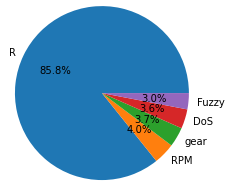
\includegraphics[width=0.50\textwidth]{figures/Data type distribution.png}
    \caption{数据类型分布图}
    \label{fig:data type distribution}
\end{figure} 

% 图\ref{fig:Histogram of raw data distribution}展示的是原始数据的分布情况,横坐标为特征的数值,纵坐标为9个特征的数量。可以发现特征"car id"与其他特征的数值差异大。因此本文将一次进行章节\ref{subsection:Data_undersampling}、\ref{subsection:Nonlinear_transformation _of_data}和\ref{subsection:Generating_images}中所述的操作。
% \begin{figure}[htb]
%     \centering
%     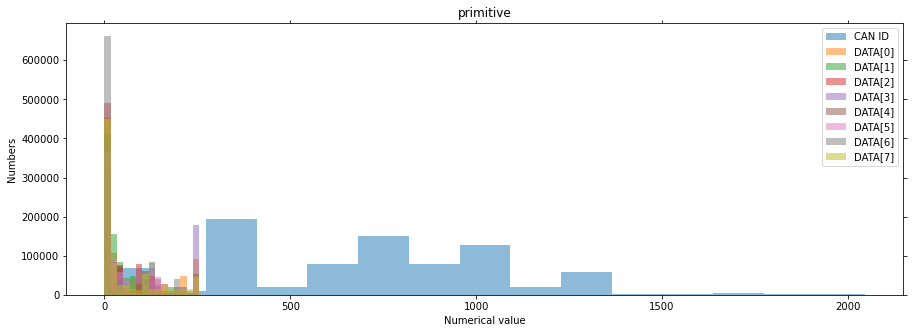
\includegraphics[width=0.8 \textwidth]{figures/Histogram of raw data distribution.png}
%     \caption{Histogram of raw data distribution}
%     \label{fig:Histogram of raw data distribution}
% \end{figure}

\textbf{评价指标及其影响因素。}\label{subsection:Evaluation_metrics_and_influencing_factors}本节针对Federated Learning(FL)中的性能问题,如准确性、延迟和资源约束等,选择了合适的评价指标,并分析了影响这些指标的因素。首先,采用F1值作为评价分类模型的准确性的指标,其定义如公式\ref{math:15}所示。F1值是精确率和召回率的调和平均,能够综合反映模型的分类效果,其值越接近1,表示模型的准确性越高。其次,本文不仅在单一深度学习模型上进行训练,还利用模型融合的方法,结合不同模型的优势,进一步提升系统的分类准确性。最后,本节考虑了入侵检测的场景和需求,将RSU作为模型的执行者,将车辆作为模型的请求者,分析了影响系统延迟和资源消耗的因素。系统延迟$T$主要由数据预处理时间$t_p$和模型训练时间$t_t$构成,而资源消耗主要包括模型的大小和算力。本节将对不同的模型进行比较和筛选,以找出适合在RSU上运行的模型。

\begin{equation}
\begin{aligned}
F1=(\frac{2+\frac{FP}{TP}+\frac{FN}{TP}}{2})^{-1}
\label{math:15}
\end{aligned}
\end{equation}

\begin{equation}
\begin{aligned}
T=t_p+t_t
\label{math:16}
\end{aligned}
\end{equation}

\textbf{数据欠采样方法的比较分析。}\label{subsection:Data_undersampling}为了解决数据不平衡问题,本节对六种数据欠采样方法进行了实验分析,分别是Random UnderSampler(RUS)、Tomek Links(TL)、One-Sided Selection(OSS)、Condensed Nearest Neighbour(CNN)、Edited Nearest Neighbours(ENN)和All-KNN,并以Near Miss(NM)作为对照组。表\ref{table:Sampling scheme and its running result}展示了各种方法的运行时间和欠采样后的样本数。从表中可以看出,基于压缩最近邻和推导的方法(CNN和OSS)在欠采样效果上较差,而基于最近邻和Tomek Links的方法(ENN、All-KNN和TL)虽然有一定的改善,但仍未能有效地解决数据不平衡问题。RUS方法虽然运行速度最快,但它只是简单地对多数类样本进行随机抽样,导致欠采样后的样本分布与原始数据分布不一致,容易造成欠拟合现象,不适用于Car-Hacking这种正负样本比例极端不平衡的数据集。综上所述,本节选择了NM方法作为最佳的欠采样方法。

\begin{table*}[!ht]
    \centering
    \caption{Sampling scheme and its running result}
    \begin{tabular}{ccccccccc}
    \hline
        \textbf{} & \textbf{Original} & \textbf{RUS} & \textbf{NM} & \textbf{TL} & \textbf{OSS} & \textbf{CNN} & \textbf{ENN} & \textbf{Allknn} \\ \hline
        $t_p$(s)  & ~ & 5.29 & 120.59 & 729.34 & 714.11 & 3526.61 & 802.87 & 2211.79 \\ 
        R & 701832 & 24624 & 24624 & 701831 & 682795 & 60 & 701824 & 701824 \\ 
        DOS & 29501 & 24624 & 24624 & 29501 & 1 & 1 & 29501 & 29501 \\ 
        RPM & 32539 & 24624 & 24624 & 32539 & 0 & 1 & 32539 & 32539 \\ 
        Gear & 29944 & 24624 & 24624 & 29944 & 1 & 1 & 29944 & 29944 \\ 
        Fuzzy & 24624 & 24624 & 24624 & 24624 & 24624 & 24624 & 24624 & 24624 \\ \hline
    \end{tabular}
    \label{table:Sampling scheme and its running result}
\end{table*}

\textbf{数据非线性转化的效果分析。}\label{subsection:Nonlinear_transformation _of_data}为了提高数据的正态性,本节对经过Near Miss降采样后的数据进行了两种不同的幂转化,分别是quantile Transformer转化和yeo-Johnson幂转化,并对转化后的数据进行了min-max标准化。图\ref{fig:Two kinds of histograms after power transformation}显示了转化后的数据直方图,从中可以发现,quantile Transformer转化能够使数据呈现出明显的高斯分布,而yeo-Johnson幂转化则没有达到这样的效果。因此,本节选择了quantile Transformer转化作为最佳的非线性转化方法。

\begin{figure}[htb]
    \centering
    \subfigure[yeo-johnson-nearmiss-maxmin]{
        \begin{minipage}[b]{1\linewidth}
        \centering
        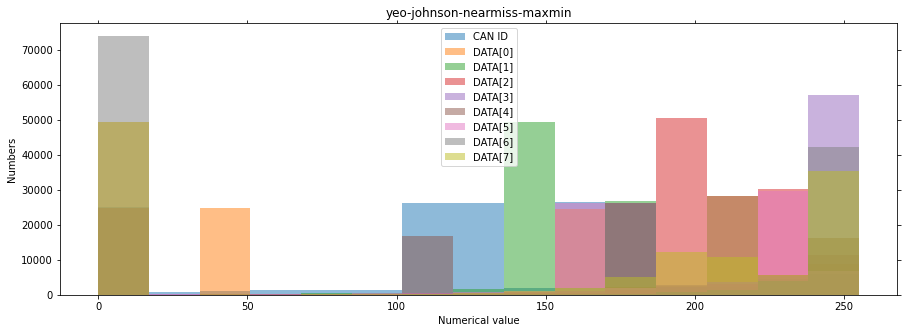
\includegraphics[width=1 \textwidth]{figures/yeo-johnson-nearmiss-maxmin.png}
        \end{minipage}
    }
    \subfigure[QuantileTransformer-normal-nearmiss-maxmin]{
        \begin{minipage}[b]{1\linewidth}
        \centering
        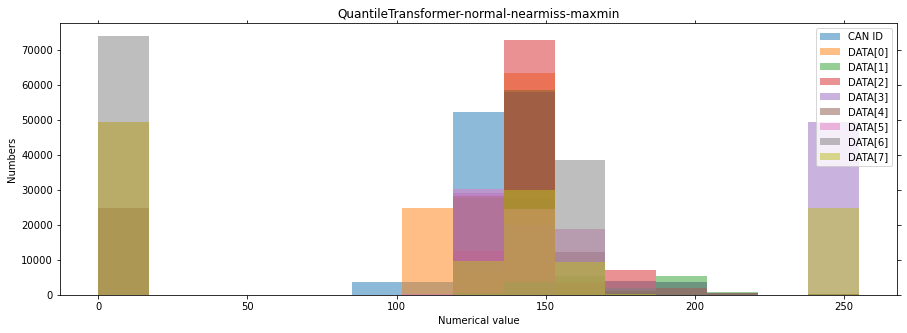
\includegraphics[width=1 \textwidth]{figures/QuantileTransformer-normal-nearmiss-maxmin.png}
        \end{minipage}
    }
    \caption{Two kinds of histograms after power transformation}
     \label{fig:Two kinds of histograms after power transformation}
\end{figure}

\subsection{实验结果与分析}\label{subsection:Generating_images}

\textbf{数据图像化的方法和效果。}\label{subsection:Data_imageization}为了适应CNN类模型的输入要求,本节将原始的文本类数据转化为图像数据。本节参考了文献\cite{A_Transfer_Learning_and_Optimized_CNN_Based_Intrusion_Detection_System_for_Internet_of_Vehicles}中的处理方案,将Car-Hacking数据集中的每条记录按照其9个特征值分别映射到一个3x3的灰度像素块上,然后将9个像素块拼接成一个9x9的大像素块。为了增加图像的信息量和多样性,本节将三个不同的9x9像素块叠加在一起,形成一个9x9的彩色图像。图\ref{fig:five picture after yeo and qtn}展示了两种不同的幂转化方法生成的图像示例。为了方便后续的CNN模型处理,本节对生成的图像进行了reshape操作,将其大小调整为224x224。

\begin{figure}[htb]
    \centering
    \subfigure[yeo-johnson-nearmiss-maxmin]{
        \begin{minipage}[b]{1\linewidth}
            \centering
            \includegraphics[width=0.9 \textwidth]{figures/yeo-johnson.png}
        \end{minipage}
    }
    \subfigure[QuantileTransformer-normal-nearmiss-maxmin]{
        \begin{minipage}[b]{1\linewidth}
            \centering
            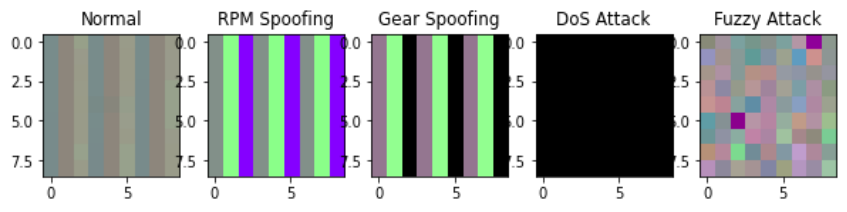
\includegraphics[width=0.9 \textwidth]{figures/quantile Transformer.png}
        \end{minipage}
    }
    \caption{Five kinds of pictures after two kinds of power transformation}
    \label{fig:five picture after yeo and qtn}
\end{figure}

\textbf{数据集划分和模型训练。}\label{subsection:Dataset_split_and_model_training}本节将生成的4395张图像数据按照8:2的比例划分为训练集和测试集,然后使用pysyft库实现联邦平均算法,定义了两个虚拟的参与者,并将训练集平均分配给他们。本节选择了一个自定义的CNN模型作为基准模型,由两个卷积层、一个最大池化层、一个平均池化层和一个全连接层组成,激活函数采用了Relu函数。使用SGD作为优化器,交叉熵作为损失函数,设置了epoch为50,Batch Size为128。图\ref{fig:FL_CNN}展示了使用yeo-Johnson幂转化和quantile Transformer幂转化后的数据进行训练的结果,可以看出,yeo-Johnson幂转化后的数据在损失函数和准确率上都有更快的收敛速度,说明本节提出的yeo-Johnson幂转化方法是有效的。

\begin{figure}[htb]
    \centering
    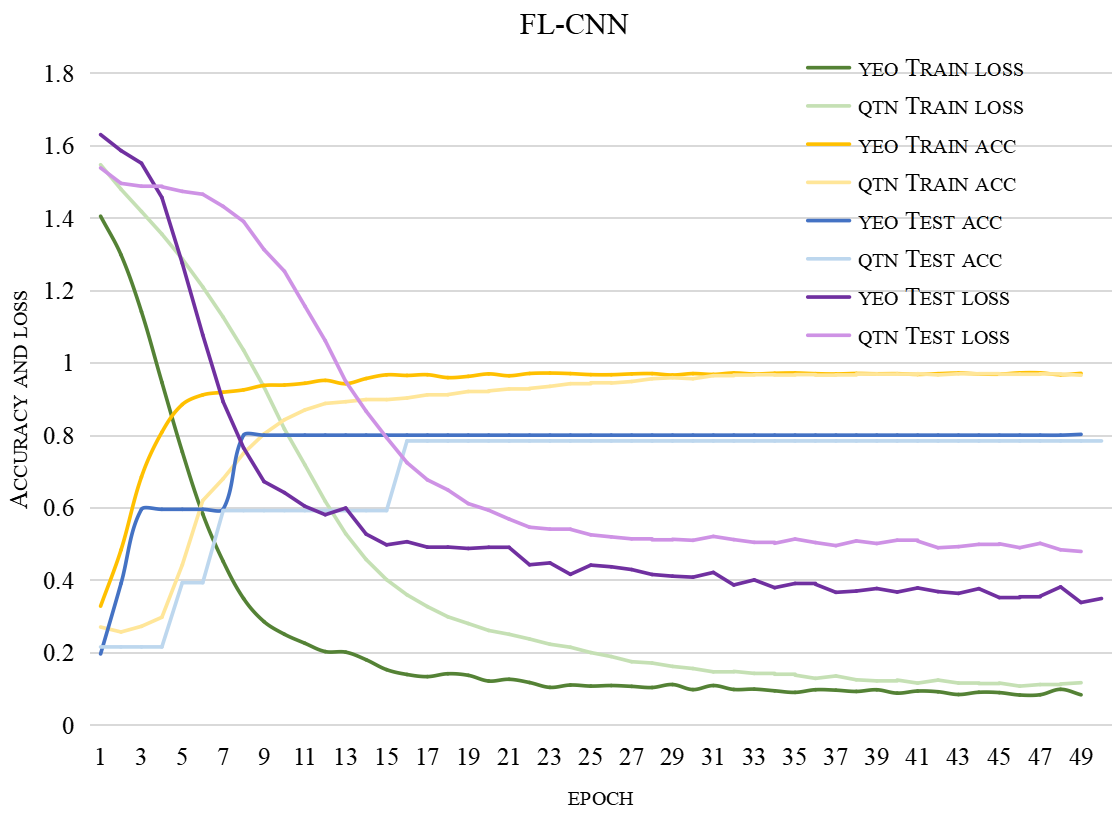
\includegraphics[width=0.45 \textwidth]{figures/FL_CNN.png}
    \caption{QuantileTransformer-normal-nearmiss-maxmin}
    \label{fig:FL_CNN}
\end{figure}

\textbf{分类结果的评估。}\label{subsection:Classification_result_evaluation}为了评估不同的CNN模型在分类任务上的性能,本节绘制了每个模型的混淆矩阵。混淆矩阵是一种常用的评价分类模型的指标,它可以在数据不平衡的情况下,直观地显示模型对每个类别的预测准确率。混淆矩阵的列代表预测的类别,行代表真实的类别。对角线上的元素表示预测正确的数量或比例,非对角线上的元素表示预测错误的数量或比例。本节期望得到的混淆矩阵是对角线上的值越大越好,表示模型能够正确地区分不同的类别。图\ref{fig:Confusion matrix of 4 types of models}显示了四种CNN模型的混淆矩阵,从中可以发现,除了ResNet18以外,其他的模型都能够较好地识别出少数类,即异常流量,只有少量的正常流量被误判为异常流量,这种情况是可以接受的,因为将异常流量误判为正常流量会带来更大的风险。ResNet18则能够完美地识别出正常流量,但是对异常流量的识别能力较差,因此本节保留了它,以备在特殊场景中使用。

\begin{figure}[htb]
\centering    
    \subfigure{
        \begin{minipage}[b]{.4\linewidth}
            \centering
            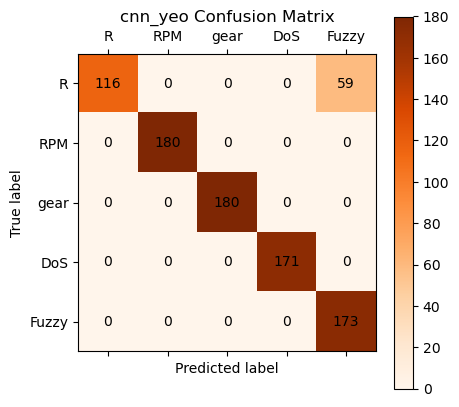
\includegraphics[scale=0.35]{figures/cnn_yeo_Confusion_Matrix.png}
            % \caption{FL-vgg16 Confusion Matrix}
        \end{minipage}
    }
    \subfigure{
        \begin{minipage}[b]{.4\linewidth}
            \centering
            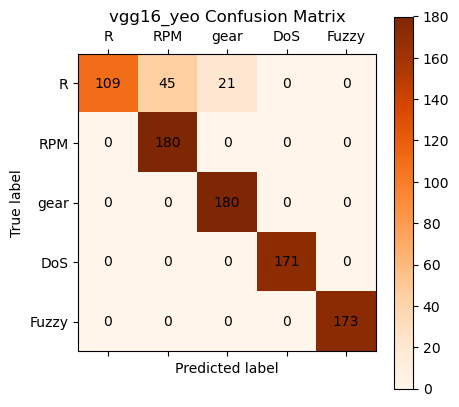
\includegraphics[scale=0.35]{figures/vgg16_yeo_Confusion_Matrix.png}
            % \caption{FL-vgg16 Confusion Matrix}
        \end{minipage}
    }

    \subfigure{
        \begin{minipage}[b]{.4\linewidth}
            \centering
            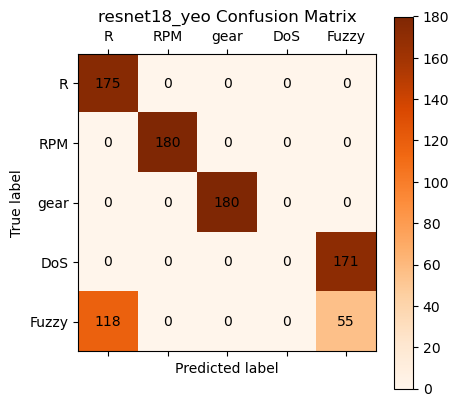
\includegraphics[scale=0.35]{figures/resnet18_yeo_Confusion_Matrix.png}
            % \caption{FL-vgg16 Confusion Matrix}
        \end{minipage}
    }
    \subfigure{
        \begin{minipage}[b]{.4\linewidth}
            \centering
            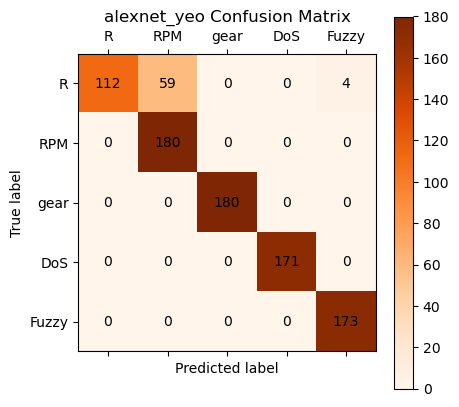
\includegraphics[scale=0.35]{figures/alexnet_yeo_Confusion_Matrix.png}
            % \caption{FL-vgg16 Confusion Matrix}
        \end{minipage}
    }
    \caption{Confusion matrix of 4 types of models}
    \label{fig:Confusion matrix of 4 types of models}
\end{figure}

\textbf{ROC曲线和AUC值的比较。}\label{subsection:ROC_curve_and_AUC_value_comparison}为了评估不同的FL模型在分类任务上的灵敏度和特异度,本节绘制了四种FL模型的ROC曲线,并计算了它们的AUC值。ROC曲线是一种用于评价二分类模型的性能的图形工具,它反映了模型的真阳性率(TPR)和假阳性率(FPR)之间的关系。AUC值是ROC曲线下的面积,它表示模型对正负样本的区分能力,其值越接近1,表示模型的性能越好。图\ref{fig:ROC curve and AUC area of five types of models}显示了四种FL模型的ROC曲线和AUC值,从中可以看出,CNN、VGG16、AlexNet模型的AUC值都达到了1,说明它们能够完美地区分正负样本,而ResNet18模型的AUC值也高达0.94,表明它也有很高的分类性能。因此,本节认为这四种FL模型都能够胜任日常的入侵检测工作。

\begin{figure}[htb]
\centering    
    \subfigure{
        \begin{minipage}[b]{.4\linewidth}
        \flushleft
        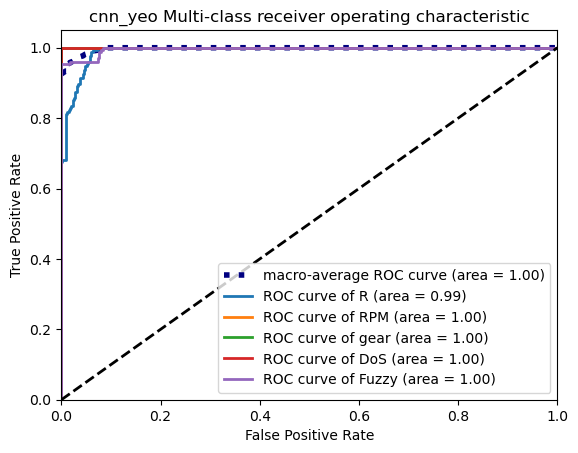
\includegraphics[scale=0.26]{figures/cnn_yeo_roc_fig.png}
        % \caption{FL-vgg16 Confusion Matrix}
        \end{minipage}
    }
    \subfigure{
        \begin{minipage}[b]{.4\linewidth}
            \flushright
            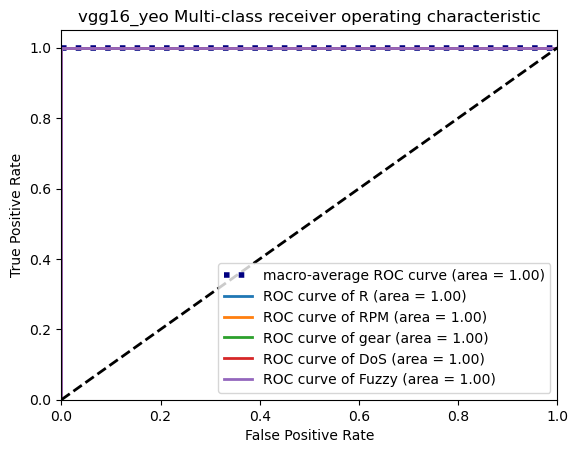
\includegraphics[scale=0.26]{figures/vgg16_yeo_roc_fig.png}
            % \caption{FL-vgg16 Confusion Matrix}
        \end{minipage}
    }

    \subfigure{
    \begin{minipage}[b]{.4\linewidth}
        \flushleft
        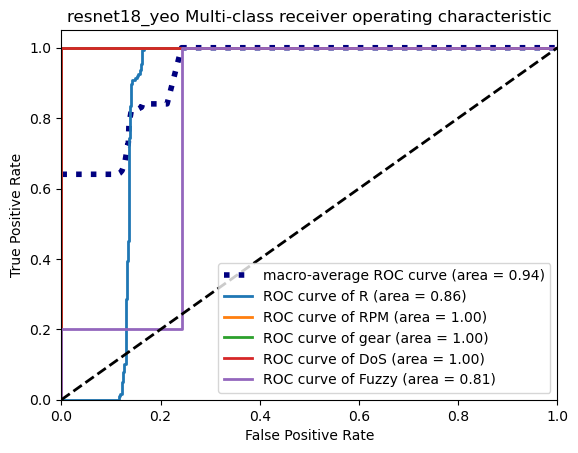
\includegraphics[scale=0.26]{figures/resnet18_yeo_roc_fig.png}
        % \caption{FL-vgg16 Confusion Matrix}
    \end{minipage}
    }
    \subfigure{
        \begin{minipage}[b]{.4\linewidth}
            \flushright
            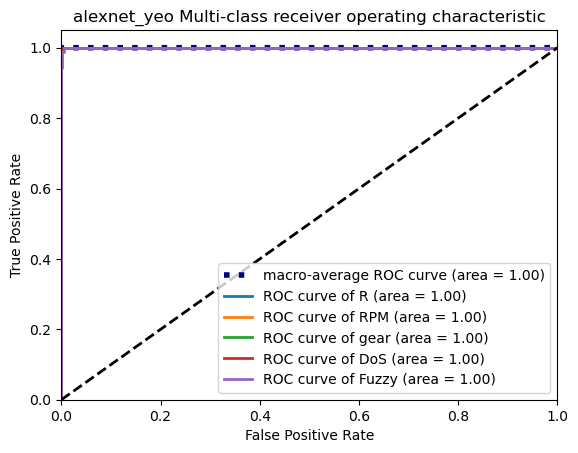
\includegraphics[scale=0.26]{figures/alexnet_yeo_roc_fig.png}
            % \caption{FL-vgg16 Confusion Matrix}
        \end{minipage}
    }
    \caption{ROC curve and AUC area of five types of models}
    \label{fig:ROC curve and AUC area of five types of models}
\end{figure}

\textbf{模型对比情况的统计分析。}\label{subsection:Model_comparison_statistics}本节对FL-CNN、FL-VGG16、FL-ResNet18、FL-AlexNet四种FL模型的性能进行了统计分析,结果如表\ref{table:Four federated learning models}所示。从表中可以看出,FL-AlexNet模型在达到最佳状态时的epoch数最少,只有10次,而其他模型都需要20次或以上。这说明FL-AlexNet模型的收敛速度较快,能够在较少的迭代次数下达到较高的准确率。另一方面,FL-CNN模型的平均训练时间最短,只有473.13秒,而FL-VGG16模型的平均训练时间最长,为712.26秒。这表明FL-CNN模型的计算效率较高,而FL-VGG16模型的计算效率较低。然而,考虑到FL模型的训练时间主要取决于参与者的网络状况和设备性能,而不是模型本身的复杂度,因此这些训练时间的差异并不显著,都在可以接受的范围内。

\begin{table}[htbp]
    \centering
    \caption{Four federated learning models}
    \begin{tabular}{ccccc}
    \hline
        \textbf{} & \textbf{FL-CNN} & \textbf{FL-VGG16} & \textbf{FL-ResNet18} & \textbf{FL-AlexNet} \\ \hline
        \text{$t_t$(s)} & 82.242301 & 713.2586751 & 244.2694107 & 146.4923077 \\ 
        \text{Best Epoch} & 9 & 3 & 34 & 5 \\ 
        \text{Size(KB)} & 222 & 524,541 & 43,725 & 222,754 \\ 
        \text{精度} & 0.932878271 & 0.924914676 & 0.671217292 & 0.928327645 \\ 
        \text{查准率P} & 0.949137931 & 0.939104478 & 0.568126491 & 0.946107841 \\ 
        \text{召回率} & 0.932571429 & 0.924571429 & 0.663583815 & 0.928 \\ 
        \text{F1 Score} & 0.930314369 & 0.920275282 & 0.604710494 & 0.925649556 \\ 
        \text{Roc\_auc R} & 0.991347403 & 1 & 0.864147727 & 1 \\ 
        \text{Roc\_auc RPM} & 1 & 1 & 1 & 1 \\ 
        \text{Roc\_auc Gear} & 1 & 1 & 1 & 1 \\ 
        \text{Roc\_auc Dos} & 1 & 1 & 1 & 1 \\ 
        \text{Roc\_auc Fuzzy} & 0.996782328 & 1 & 0.806792317 & 0.999885376 \\ \hline
    \end{tabular}
    \label{table:Four federated learning models}
\end{table}

\section{本章小结}

本章介绍了一种基于迁移学习和特征工程的联邦学习CAN异常检测设计框架。MEC作为边缘计算平台,负责对来自不同RSU的联邦模型进行聚合更新和数据存储。RSU作为车联网的核心节点,负责本地模型的训练、数据收集、清洗和异常检测执行,并将检测结果反馈给所属区域的车辆。RSU根据车辆识别码(VIN)对区域内的车辆进行K-means聚类,从每个类别中选择$k \geq 1$辆车作为本地数据来源。为了在智能车上实现入侵检测,本章采用了轻量级的DL模型和欠采样技术,以降低计算资源消耗并解决样本不均衡的问题。此外,引入了特征工程思想,对数据进行了非线性变换(yeo-Johnson变换),然后使用min-max标准化将数据缩放到$0-1$之间。迁移学习的思想也被引入,利用多个领域的共享知识来建立有效的模型。MEC中集成四类预训练后的DL模型,分别是CNN、VGG16、ResNet18和AlexNet。在系统启动的初期,MEC会将这四类模型下发给选中的$\alpha$个RSUs。最后,研究了在移动边缘计算(MEC)环境下,如何为不同类型的路侧单元(RSU)提供个性化的深度学习(DL)模型,以实现车辆入侵检测的联邦学习任务。MEC作为系统的中心节点,负责模型的聚合与分发。整个系统将一直重复这个过程,直到$g_{t+1}$收敛。MEC将持续监控达到收敛状态的全局模型,一旦发现由于车辆移动导致的RSU收集到的CAN数据变化、特殊RSU离线等原因导致模型检测性能下降,将再次重启整个联邦学习过程。

% 随着智能车辆的功能越来越多,其暴露出来的脆弱点也在增多。当这些暴露出来的脆弱面被攻击者恶意利用时,会给用户及企业带来隐私泄露、功能故障、财产损失甚至生命威胁。本节发现车联网中存在的安全问题具有高度的动态性、复杂性和隐蔽性等特点。针对动态性,本节提出将IDS的主动权交给静态的RSU,而不断移动的车辆为被检测者,本节提出将CP-ABE加密策略应用于RSU与车之间的数据交换,在保障网络交换效率的同时兼顾了数据信息安全。针对车联网攻击的复杂性和隐蔽性,本节提出迁移学习结合联邦学习技术进行入侵检测。接下来本节将从车联网外攻击扩展到车联网内外的攻击,以此来探究本节提出的模型是否具有普适性。